\subsection{Apresentação do problema}

%SLIDE DE APRESENTAÇÃO DO PROBLEMA
\begin{frame}
\frametitle{Apresentação do problema}
\begin{itemize}
    \item O posicionamento dos instrumentos dentro do túnel de vento é realizado de forma manual, exigindo que o operador desligue o túnel.
    \item Isso causa uma baixa repetibilidade e menor precisão. 
    \item Para tanto, propomos o desenvolvimento de um mecanismo que faça esse deslocamento dos instrumentos de medição de forma automatizada.
\end{itemize}
\end{frame}

\begin{frame}
    \frametitle{Apresentação do problema}
        \begin{figure}
        \centering
        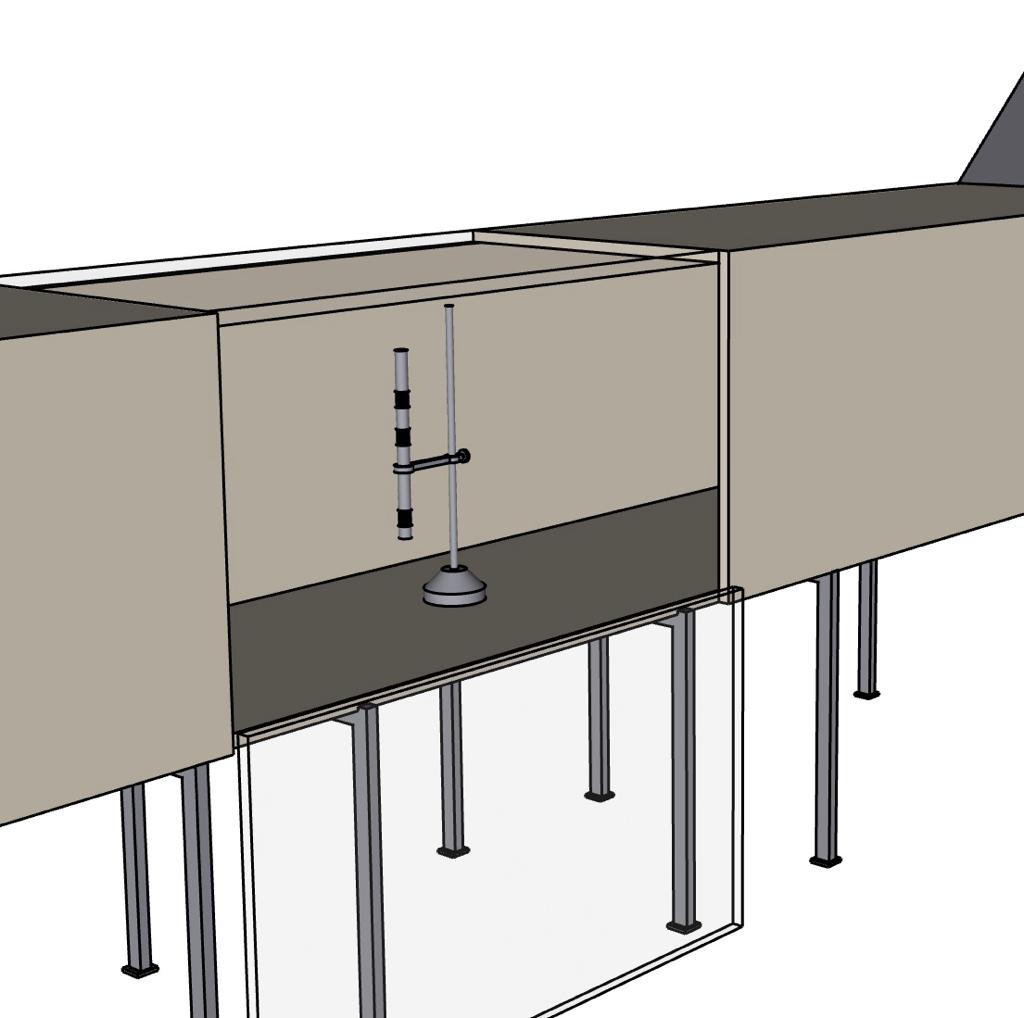
\includegraphics[scale = 0.15]{figuras/sisantigozoom}
        \end{figure}
\end{frame}
    